\hypertarget{part-1-design-4}{%
\section{Part 1, design 4}\label{part-1-design-4}}

\centering
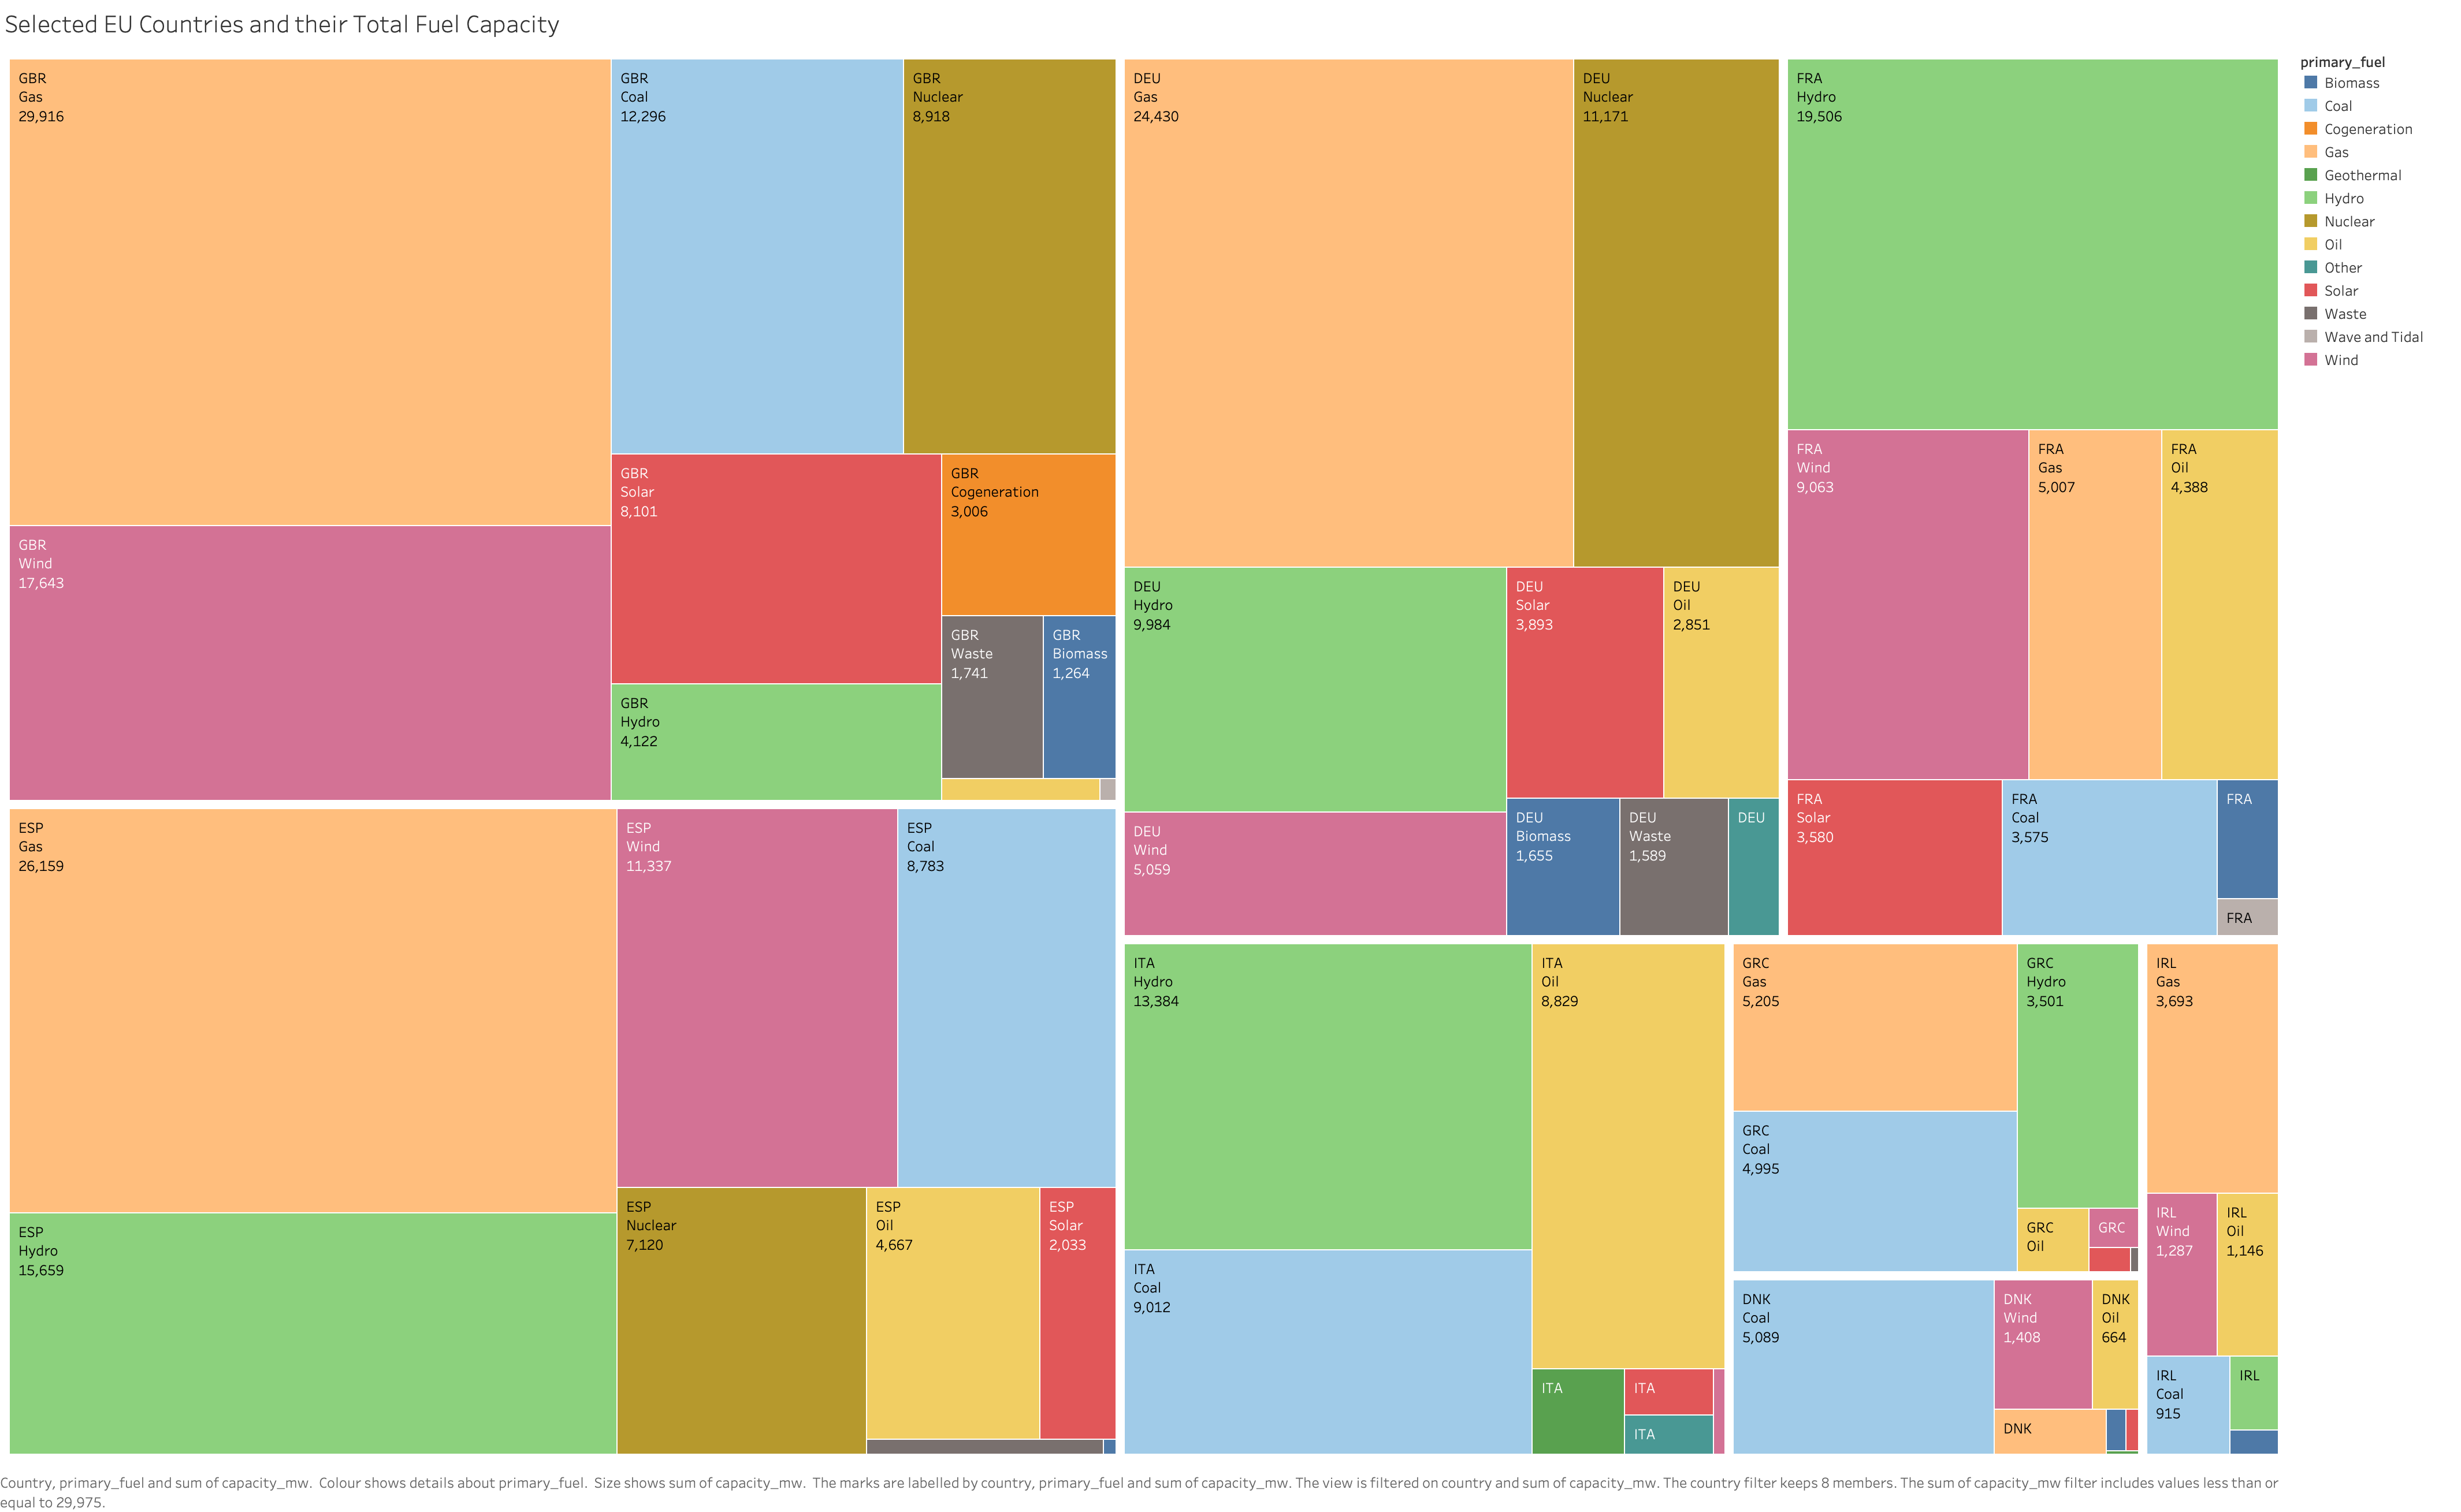
\includegraphics[width=15cm]{Viz4.png}

\hypertarget{description}{%
\subsubsection{Description}\label{description}}

\begin{description}
\item[Visual Design Type:]
Treemap
\item[Name of Tool:]
Tableau
\item[Country:]
Great Brittan, Spain, Germany, Italy, France, Greece, Denmark, Ireland.
\item[Year:]
2018
\item[Visual Mappings:]
\begin{itemize}
	\tightlist
	\item[  ]
\end{itemize}

\begin{itemize}
\tightlist
\item
  \textbf{mapping 1}: Primary fuel was used for the colour coding.
\end{itemize}
\begin{itemize}
	\tightlist
	\item
	\textbf{mapping 2}: sum of the capacity was used for the size.
\end{itemize}
\begin{itemize}
\tightlist

\item
  \textbf{mapping 3}: Country, primary fuel and sum of the capacity was used as a label within the visualisation.
\end{itemize}
\item[Unique Observation:]
France has the most amount of energy capacity. The largest of the capacity being for nuclear energy with a capacity of 63,130. The country with the next amount of capacity is Germany with Coal being its primary fuel at 47,773.
\item[Data Preparation:]
A filter on the countries listed has been used.
\end{description}
 
